\section{Introduction}


Deep learning has been transformative for a variety of fields such as natural language processing~\citep{devlin2018bert}, computer vision~\citep{krizhevsky2012imagenet}, geometry processing~\citep{qi2017pointnet}, and 3D vision~\citep{deng2018ppfnet}. This rapid proliferation has brought with it surprising phenomena that defy the predictions of classical statistical learning theory.


In this paper we explore one such recently observed phenomenon known as \emph{grokking}, first described by \citet{power2022grokking} as a sudden and unexpected generalization occurring after prolonged overfitting. Although predominantly studied in algorithmic tasks like modular addition or multiplication, recent findings suggest that grokking may be a more pervasive phenomenon, also manifesting in more complex tasks involving vision and language~\citep{lv2024language,humayun2024deep}.


Prior research has consistently observed grokking in settings that involve some form of regularization, such as weight decay~\citep{Barak2022-el, power2022grokking, Nanda2023-hf}. This pattern has motivated investigations into the implicit biases introduced by weight decay, suggesting it may be critical to triggering delayed generalization. For instance, \citet{liu2023omnigrok} argued that weight norms need to be in a narrow range or ``Goldilocks Zone'' for generalization. Similarly, \citet{Varma2023} highlighted weight efficiency of generalizing solutions, and \citet{Nanda2023-hf} argued that weight decay favors simpler, more generalizable solutions. However, recent works have argued that regularization may not be necessary for grokking, at least on shallow networks with Mean Squared Error (MSE) loss \citep{Kumar2023-hz, Lyu2023-ga, Gromov2023-nh}. These works tie grokking to a transition from lazy training \citep{Chizat_Oyallon_Bach_2018} to feature learning. Despite this ongoing work, several aspects in this framing of grokking remain unclear. These include why grokking tasks induce lazy training and why weight decay is often needed to enter the feature learning regime when using deeper models or cross-entropy (CE) loss.


Here we propose a novel account of grokking, outlined in \cref{fig:teaser}, that explains several of the main unanswered questions in the grokking literature. We start by showing that without regularization, grokking is prevented by absorption errors in the \softmax, which we call \emph{Softmax Collapse} (SC). These errors result in zero terms in the gradient and put an end to learning, sometimes before any progress is made in the test performance, resulting in complete overfitting (\cref{fig:teaser}, \textbf{c}). We then argue that SC is caused by what we call \emph{Naïve Loss Minimization} (NLM), as the gradient becomes aligned with a direction that corresponds to scaling up the logits by a constant. While scaling up all the logits does not change the model predictions, it does reduce the CE loss for a network that has reached 100\% training accuracy, with the downside that this eventually leads to numerical errors in \softmax. 
Our findings provide explanations for several key aspects of grokking, including (i) the delayed onset of generalization, (ii) why grokking is often absent without regularization, and (iii) why existing methods designed to induce grokking are effective.

To validate our hypothesis that SC is responsible for the absence of grokking without regularization, we introduce $\bm{\stablemax}$ as a more numerically stable replacement to $\softmax$ in CE loss. This simple change takes models from complete overfitting to grokking (\cref{fig:teaser}, \textbf{c} to \textbf{b}) \textit{without} regularization, in settings where it is normally not observed without it. Similarly, we validate that NLM is responsible for delaying generalization (\cref{fig:teaser}, \textbf{a} to \textbf{b}) and leading to SC by introducing a new optimizer $\ograd$, which only preserves the part of the gradient that is orthogonal to the NLM direction. By doing this, $\ograd$ quickly leads to generalization without the initial overfitting phase that defines grokking (\cref{fig:teaser}, \textbf{b} to \textbf{a}).

Our primary contributions are as follows:
\begin{itemize}[leftmargin=*,topsep=0em,noitemsep]
    \item We observe that cases of overfitting without grokking are due to floating point errors caused by extreme values in the $\softmax$~function, which we term Softmax Collapse (SC;~\cref{sec:floating_points}).
    \item We show that interventions to avoid SC, like greater floating point precision or a new, numerically stable version of Softmax ($\stablemax$), cause grokking in settings where it was previously absent without regularization (\cref{sec:preventing_sc}).
    \item We observe that models move towards SC because overfitting and cross-entropy loss push the model in a direction of uncontrolled logit growth, which we refer to as Naïve Loss Minimization (NLM;~\cref{sec:nlm}).
    \item We demonstrate that NLM can be avoided through a novel optimizer, \ograd, which removes the delay in generalization (\cref{sec:avoiding_nmm}).
\end{itemize}


\begin{figure}[t]
\begin{centering}
    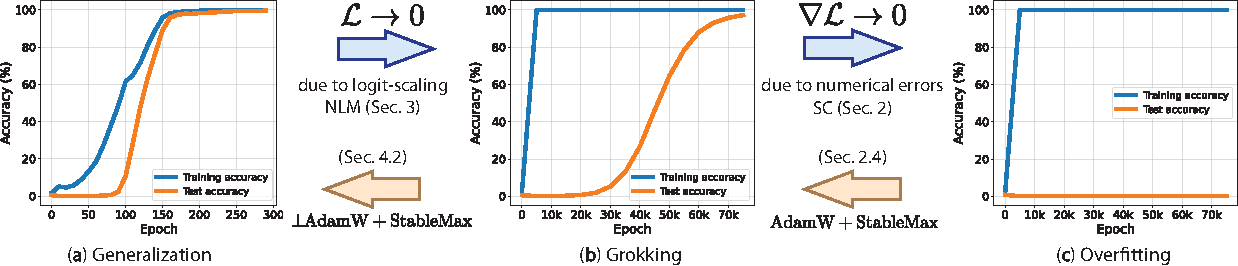
\includegraphics[width=\linewidth]{grokking_iclr_arxiv/figures/grokking.pdf}\vspace{-6mm}
\end{centering}
\caption{Our contributions demonstrated through results obtained in addition modulo 113 task. We show that the delay in generalization induced by NLM can be reversed using the proposed $\perp$\!AdamW ((\textbf{a}) and (\textbf{b})) and that the numerical errors that lead to overfitting instead of grokking can be avoided by using the proposed $\stablemax$ ((\textbf{b}) and (\textbf{c})). \vspace{-5mm}}
\label{fig:teaser}
%\vspace{-3mm}
\end{figure}

\begin{comment}
\begin{figure}[t]
\begin{subfigure}[t]{.32\textwidth}
    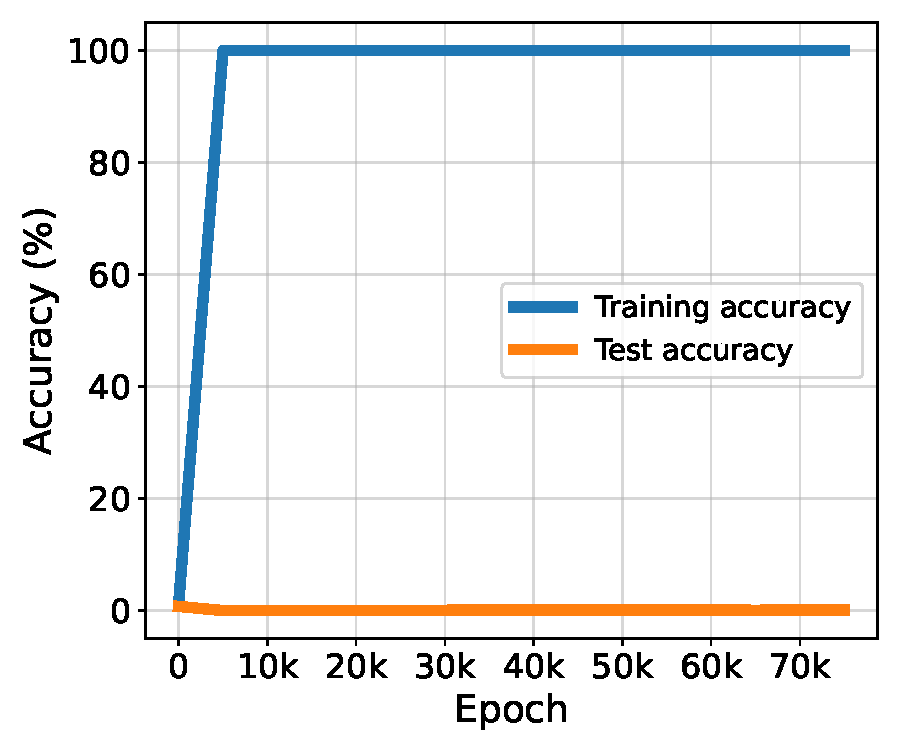
\includegraphics[width=\linewidth]{grokking_iclr/figures/teaser_baseline.pdf}
    \caption{AdamW}
\end{subfigure}
\hfill
\begin{subfigure}[t]{.32\textwidth}
    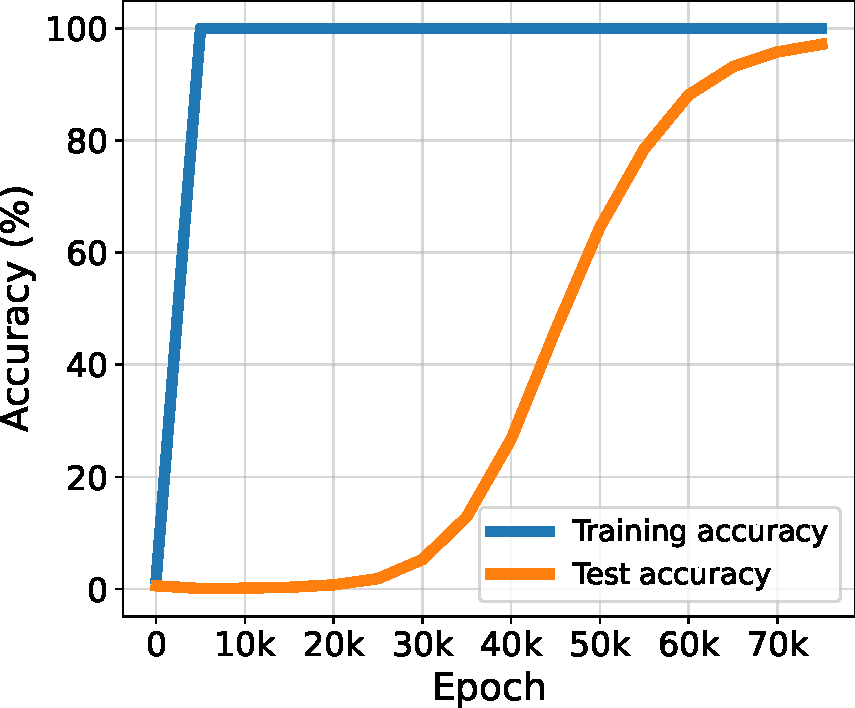
\includegraphics[width=\linewidth]{grokking_iclr/figures/teaser_softermax.pdf}
    \label{fig:input_representations}
    \caption{AdamW + stablemax}
\end{subfigure}%
\hfill
\begin{subfigure}[t]{.32\textwidth}
    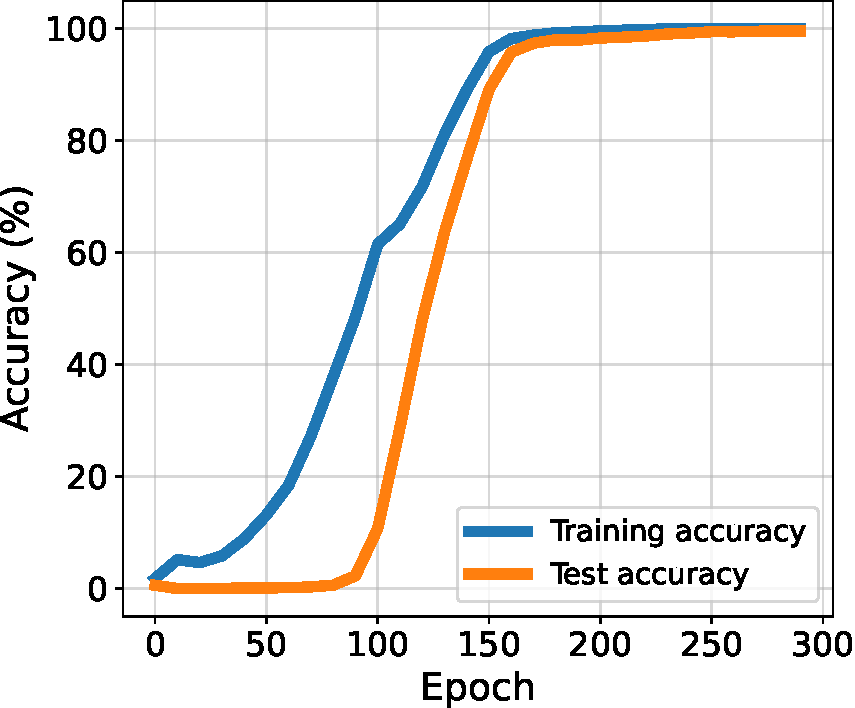
\includegraphics[width=\linewidth]{grokking_iclr/figures/teaser_nlm.pdf}
    \label{fig:gradient_norms}
    \caption{$\perp$AdamW + stablemax}
\end{subfigure}
\caption{\vspace{-5mm}}
\vspace{-5mm}
\end{figure}
\end{comment}